\documentclass[12pt]{article}

\usepackage[utf8]{inputenc}
\usepackage[greek, english]{babel}
\usepackage{alphabeta}
\usepackage{libertine}
\usepackage{graphicx}

%\pagenumbering{gobble}
\title{1o ΣΕΤ ΑΣΚΗΣΕΩΝ \\ ΑΛΓΟΡΙΘΜΟΙ}
\author{ΤΖΕΝΗ ΜΠΟΛΕΝΑ 3170117}
\date{}

\begin{document}
	
\maketitle
	
  \section{\underline{Άσκηση 1 Binary Search}}
  \subsection{Τρόπος υλοποίησης}
  Η υλοποίηση είναι ίδια με αυτή της απλής binary search , με τη διαφορά ότι δεν σταματάμε με το που βρούμε για πρώτη φορά το στοιχείο. Επειδή θέλουμε να βρούμε και την πρώτη και τελευταία εμφάνιση του στοιχείου περνάμε σαν όρισμα στην μέθοδο μας πιό θέλουμε να βρούμε και αναλόγως αυτό με βάση τις συνθήκες βρίσκει την πρώτη ή τελευταία εμφάνηση. Αν το στοιχείο προς αναζήτηση δεν υπάρχει τότε επιστρέφεται $-1$ .  Στην ουσία όταν θέλουμε να βρούμε την πρώτη εμφάνιση κάνουμε κανονική Binary search με τη μόνη διαφορά όταν βρούμε το στοιχείο συνέχιζουμε να ψάχνουμε στον αριστερό υποπίνακα γαι να δούμε αν το στοιχείο εμφανίζεται σε κάποια προηγούμενη θέση του πίνακα. Ομοίως όταν θέλουμε να βρούμε την τελευταία εμφάνιση, με τη διαφορά οτι όταν το βρούμε συνεχίζουμε και ψάχνουμε στο δεξί υποπίνακα.
  
  \subsection{Πολυπλοκότητα}
  Η μαθηματική συνάρτιση που εκφράζει την Binary Search είναι: \\ $T(n) = T(n/2) + 1$ \\
  Με χρήση θεωρήματος Master έχουμε $ a=1$ και $b=2$ οπότε $\log_{2}1 = 0$. \\ Άρα $n^0 = 1$ , οπότε είμαστε στην δευτερή περίπτωση του θεωρήματος Master και έχουμε πολυπλοκότητα  $\Theta(\log_{}n)$! Την binary search την καλούμε δυο φορές, μία για την πρώτη εμφάνιση και μία για την τελευταία, οπότε για  να είμαστε ακριβείς έχουμε πολυπλοκότητα $\Theta(2\log_{}n)$, άρα $\Theta(\log_{}n)$.
  
  \subsection{Οδηγείες για εκτέλεση προγράμματος}
  Για να τρέξει το πρόγραμμα πρέπει να δωθούν ως ορίσματα το όνομα του αρχείου απο το οποίο διαβάσουμε τα στοιχεία και επίσης χρειάζεται να δωθεί και το στοιχείο πάνω στο οποίο θα γίνει αναζήτηση. Συγκεκριμένα στο $args[0]$ πρέπει να έχουμε το path του αρχείου και το $args[1]$ πρέπει να έχουμε το στοιχείο προς αναζήτηση.
  \\ \\ \\
   
  \section{\underline{Άσκηση 2 QuickSort}}
  \subsection{Τρόπος υλοποίησης}
  Ξεκινάμε καλώντας την quickSort απο το main program και κάνουμε διαμέρηση στον πίνακα μας(quickSort καλεί partition) και ξέρουμε πως μετά απο κάθε διαμέριση(partition) όλα τα στοιχεία ίσα με το pivot βρίσκονται στη σωστή θέση, οπότε μετά χρειάζεται να καλέσουμε τη quickSort για τα στοιχεία αριστερά της πρώτης εμφάνησης του pivot(στοιχεία μικρότερα του pivot) και για τα στοιχεία δεξιά της τελευταίας εμφάνησης του pivot(στοιχεία μεγαλύτερα του pivot)... .Ας δούμε λίγο πιο αναλυτικά πως λειτουργεί η partition. Το σκεπτικό είναι απλό. Έχουμε την αρχή και το τέλος του πίνακα όπου θα κάνουμε διαμέριση και έχουμε και μια έξτρα μεταβλητή(visitIndex) με την οποία διασχίζουμε τον πίνακα. Την μεταβλητή αυτήν την αρχικοποιούμε με την αρχή του πίνακα(υποπίνακα).Στη συνέχεια ελέγχουμε αν η τιμή της θέσης που δίχνει η visitIndex είναι μικρότερη του pivot, αν ναι τότε το αλλάζουμε με την αρχή του πίνανα ετσί ώστε τα στοιχεία μικρότερα του pivot να είναι αριστερά του, επιπλέον το visitIndex αυξάνεται  κατα ενα καθώς και το σημείο που θεωρούμε αρχή του πίνακα, αφού εκεί πλέον βρίσκεται στοιχείο μικότερο του pivot.  Αν η τιμή της θέσης που δίχνει η visitIndex δεν είναι μικρότερη του pivot τσεκάρουμε αν είναι ιση, αν ναι τότε δεν υπάρχει λόγος να κάνουμε κάποια αλλαγή και απλά μεταβάλουμε το visitIndex κατα ένα για να ελέξουμε το περιεχόμενο του επόμενου κελιού. Αν δεν ισχύει κανένα απο τα παραπάνω σημαίνει οτι το στοιχείο στο οποίο δείχνει το visitIndedx ειναι μεγαλύτερο του pivot. Τότε γίνεται μια απλή αλλαγή του με το στοιχείο στο τέλος του πίνακα και μειώνουμε αυτό που θεωρούμε τέλος του πίνακα μας κατα ενα, αφού απο αυτο το σημείο αυτό και έπειτα τα στοιχεία είναι μεγαλύτερα του pivot. Η διαδικασία αυτη επαναλαμβάνεται έως ότου το visitIndex φτάσει μεχρι και το end του πίνακα(το end του πίνακα το μειώνουμε αναλόγως τη συνθήκη που έχουμε, αλλα αυτο είναι απλα μια μεταβλητή, δεν σημαίνει οτι πειράζουμε το μέγεθος του πίνακα), δλδ τότε είμαστε σίγουροι ότι έχει γίνει σωστός διαχωρισμός. Στην class QuickSort έχω εναν static πίνακα με δυο θέσεις απο integers όπου κάθε φορά όταν τελειώνει το partition, βάζω τις θέσεις με τις οποίες θα καλεστεί η quickSort γαι να γινει ξανά partition. \\
  
  \subsection{Πολυπλοκότητα}
  \begin{itemize}
  \item Worst case complexity: $\mathcal{O}(n^2)$
  \item Average case complexity:$\Theta(n\log_{}n)$.
  \item Best case complexity:$\Omega(n)$
  \end{itemize}
  
  Ας δούμε γιατί η χειρότερη περίπτωση είναι  $\mathcal{O}(n^2)$
  \begin{center}
     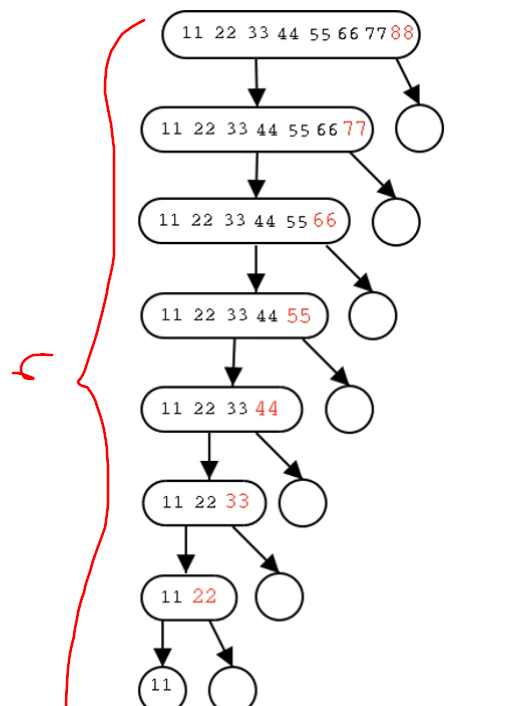
\includegraphics[scale = 0.7]{quick_image.png}
  \end{center}
   Από την παραπάνω εικόνα βλέπουμε την χειρότερη περίπτωση της quickSort. Ο πίνακας είναι ήδη ταξινομημένος και σαν pivot επιλέγεται το τελευταίο στοιχείο. Οπότε κάθε φορά που κάνουμε partition ο πίνακας δεν σπάει στα δυο. Επομένως έχουμε $height = n$ και η partition έχει πολυπλοκότητα $\mathcal{O}(n)$ οπότε συνολική πολυπλοκότητα quickSort είναι  $\mathcal{O}(n^2)$. Η μέση  περίπτωση είναι $\Theta(n\log_{}n)$. Η καλύτερη είναι $\Omega(n)$
   αφου αν τα στοιχεία του πίνακα είναι όλα ίδια τότε η partition θα γίνει μόνο μια φορά. Στην ουσία ολα τα στοιχεία θα είναι ίδια με το pivot οπότε με τα indexes που θα επιστραφούν η quicksort δεν θα ξανακαλεστεί.
  

  
  \subsection{Οδηγείες για εκτέλεση προγράμματος}
   Για να τρέξει το πρόγραμμα πρέπει να δωθεί ως ορίσματα το όνομα του αρχείου απο το οποίο διαβάσουμε τα στοιχεία.  Συγκεκριμένα στο $args[0]$ πρέπει να έχουμε το path του αρχείου. 
	
\end{document} 